\documentclass[aspectratio=169, 10pt]{beamer}

\usepackage{wrapfig}
\usepackage{tikz}
\usepackage{pgfplots}
\usetikzlibrary{positioning}

\setbeamertemplate{footline}[frame number]

\title{TicTacCoAP}
\subtitle{Advanced Technologies in the IoT – Project}
\author{Lena Boeckmann (\texttt{lena.boeckmann@haw-hamburg.de})\\Timo Kuhlbrodt (\texttt{timo.kuhlbrodt@haw-hamburg.de})}
\date{\today}

\begin{document}
    \frame{\titlepage}
    \begin{frame}
        \frametitle{Die Idee}
        \begin{itemize}
            \item TicTacToe-Spiel auf der Konsole
            \item Steuerungsinput durch phyWAVE-KW22 Boards
            \item Auslesen eines Bewegungssensors über CoAP
        \end{itemize}
    \end{frame}

    \begin{frame}
        \frametitle{Hardware}
        \begin{columns}{}
            \column{0.5\textwidth}
            \begin{itemize}
                \item Raspberry Pi
                \item Zwei phyWAVE-KW22 Boards mit Beschleunigungssensor
            \end{itemize}
            \column{0.5\textwidth}
            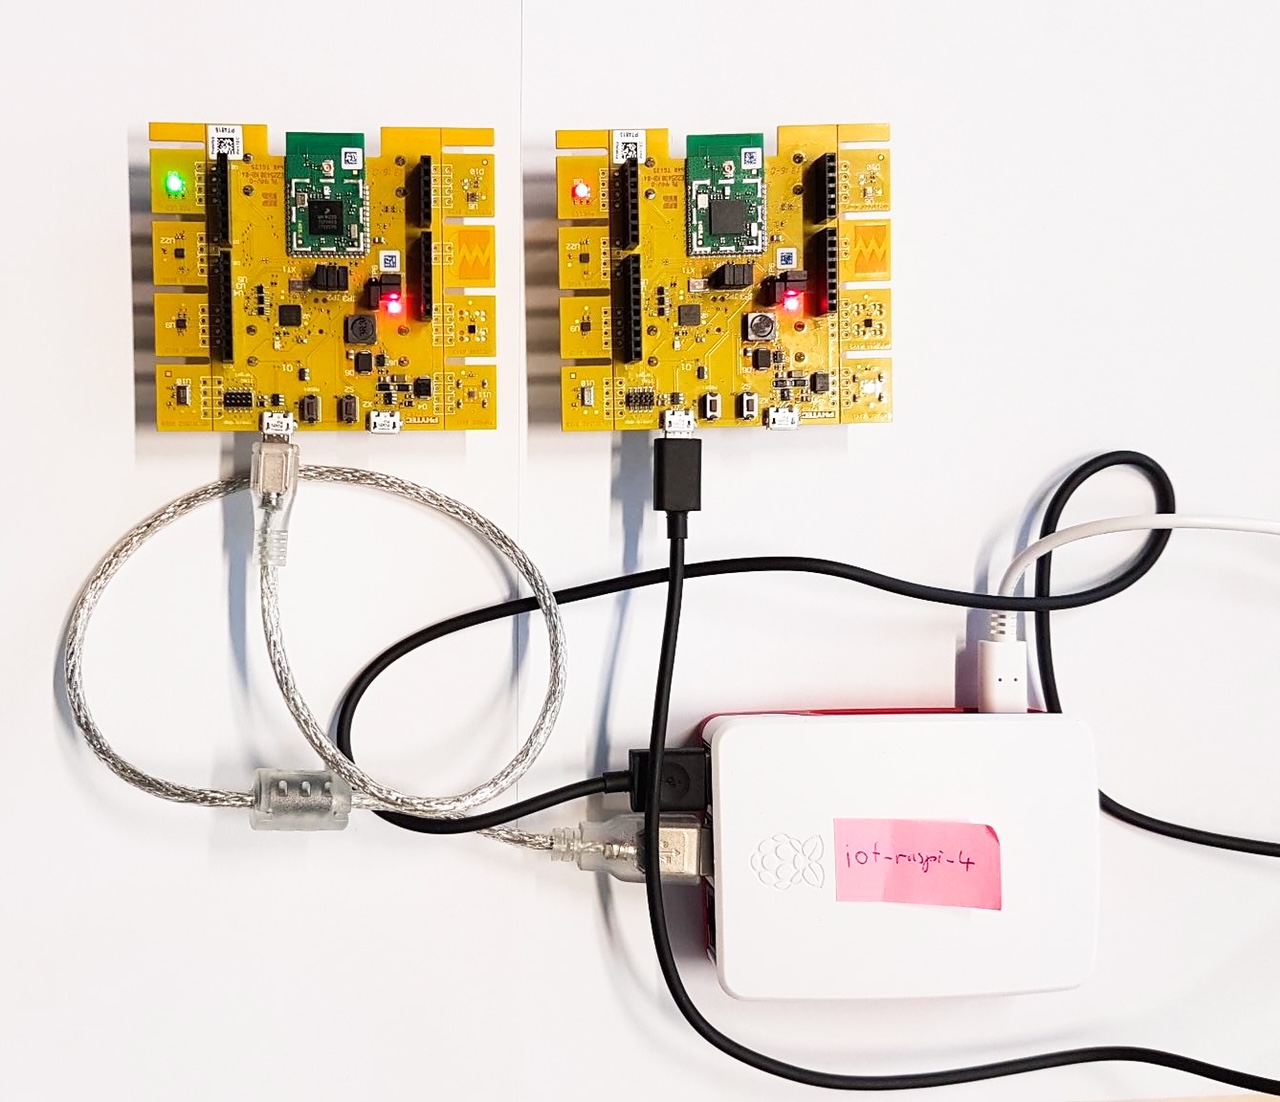
\includegraphics[width=0.9\textwidth]{figs/setup.jpg}
        \end{columns}

    \end{frame}

    \begin{frame}
        \frametitle{Software}
        \begin{columns}
            \column{0.5\textwidth}
            \begin{itemize}
                \item CoAP-Server auf den phyWAVE Nodes
                \item Python Script liest über CoAP Beschleunigungssensor aus
                \item Position der Nodes steuern den Cursor\\und setzen X/O
                \item Visualisierung im Terminal\\mit Curses Library
            \end{itemize}
            \column{0.5\textwidth}
            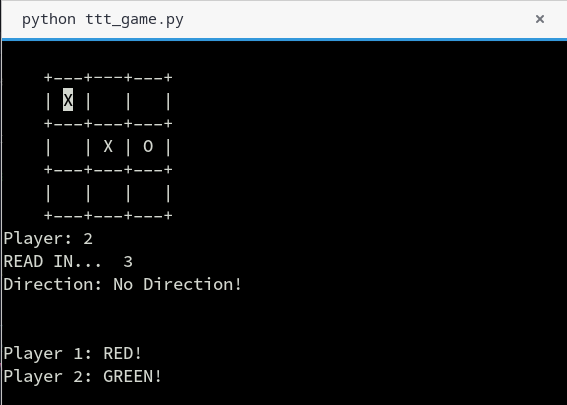
\includegraphics[width=0.9\textwidth]{figs/game.png}
        \end{columns}
    \end{frame}

    \begin{frame}
        \centering
        \textbf{Live Demo}
    \end{frame}
\end{document}